% Source: graduate-coursework/Research/How_to_write/00_Contrastive_Synthesis.tex
% Description: Radar chart comparing six major writing theories across the six axes of contrast identified in this paper. Each theory's ``footprint'' reflects its characteristic emphases. Outward position indicates stronger identification with the labeled pole (e.g., farther on the Activity axis means more activity-oriented; farther on the Reader axis means more reader-centered). Note that no single theory spans all dimensions equally, illustrating why a composite approach is necessary.

\documentclass[border=4pt]{standalone}
\usepackage{newtxtext,newtxmath}
\usepackage{tikz}
\usetikzlibrary{arrows.meta,positioning,shapes.geometric,calc,decorations.pathreplacing}

\definecolor{garnet}{HTML}{73000A}
\definecolor{atlantic}{HTML}{466A9F}
\definecolor{congaree}{HTML}{1F414D}
\definecolor{horseshoe}{HTML}{65780B}
\definecolor{rose}{HTML}{CC2E40}
\definecolor{honeycomb}{HTML}{A49137}
\definecolor{warmgrey}{HTML}{676156}
\definecolor{black90}{HTML}{363636}
\definecolor{black70}{HTML}{5C5C5C}
\definecolor{black50}{HTML}{A2A2A2}
\definecolor{black30}{HTML}{C7C7C7}
\definecolor{black10}{HTML}{ECECEC}
\definecolor{sandstorm}{HTML}{FFF2E3}

\begin{document}
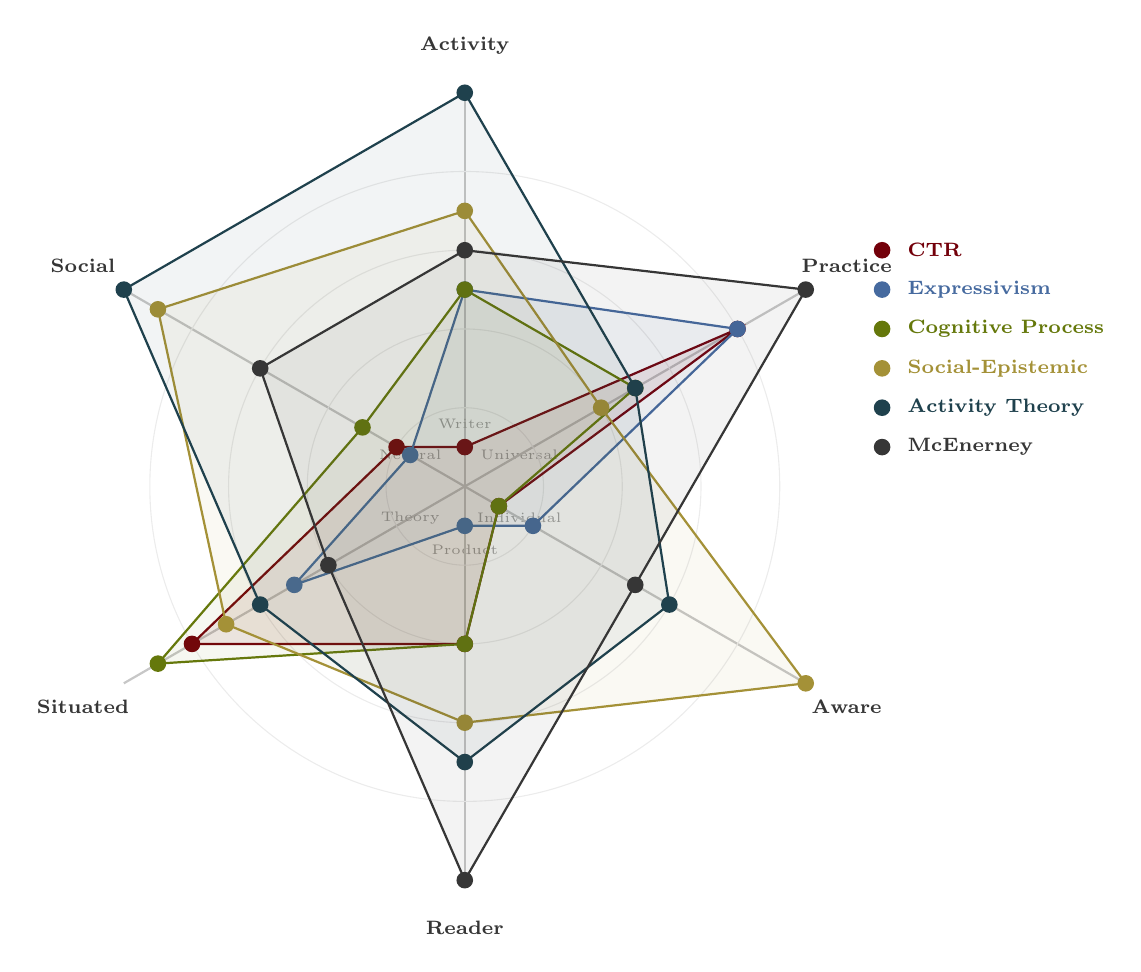
\begin{tikzpicture}[
    every node/.style={font=\scriptsize},
    axislabel/.style={font=\scriptsize\bfseries, text=black90},
    dot/.style={circle, inner sep=0pt, minimum size=6pt},
]

% Axes
\def\axislen{5.0}
\def\naxes{6}

% Axis labels and endpoints
\def\axes{
    {90/Product--Activity/Product/Activity},
    {150/Individual--Social/Individual/Social},
    {210/Universal--Situated/Universal/Situated},
    {270/Writer--Reader/Writer/Reader},
    {330/Ideology-Neutral--Aware/Neutral/Aware},
    {30/Theory--Practice/Theory/Practice}%
}

% Draw axes
\foreach \angle/\name/\labela/\labelb in \axes {
    \draw[thick, black30] (0,0) -- (\angle:\axislen);
    \node[axislabel] at (\angle:\axislen+0.6) {\labelb};
    % Inner label
    \node[font=\tiny, text=black50] at (\angle+180:0.8) {\labela};
}

% Grid circles
\foreach \r in {1,2,3,4} {
    \draw[thin, black10] (0,0) circle (\r cm);
}

% Helper macro: plot a theory as connected polygon
% Arguments: color, name, and 6 values (0-5 scale for each axis)
% Axis order: Product-Activity, Individual-Social, Universal-Situated,
%             Writer-Reader, Neutral-Aware, Theory-Practice

% CTR: product, individual, universal, writer-ish, neutral, practice
\draw[thick, garnet, fill=garnet, fill opacity=0.08]
    (90:0.5) -- (150:1) -- (210:4) -- (270:2) -- (330:0.5) -- (30:4) -- cycle;
\foreach \angle/\r in {90/0.5, 150/1, 210/4, 270/2, 330/0.5, 30/4} {
    \node[dot, fill=garnet] at (\angle:\r) {};
}

% Expressivism: process, individual, somewhat situated, writer, neutral, practice
\draw[thick, atlantic, fill=atlantic, fill opacity=0.06]
    (90:2.5) -- (150:0.8) -- (210:2.5) -- (270:0.5) -- (330:1) -- (30:4) -- cycle;
\foreach \angle/\r in {90/2.5, 150/0.8, 210/2.5, 270/0.5, 330/1, 30/4} {
    \node[dot, fill=atlantic] at (\angle:\r) {};
}

% Cognitive Process: process, individual, universal, balanced, neutral, balanced
\draw[thick, horseshoe, fill=horseshoe, fill opacity=0.06]
    (90:2.5) -- (150:1.5) -- (210:4.5) -- (270:2) -- (330:0.5) -- (30:2.5) -- cycle;
\foreach \angle/\r in {90/2.5, 150/1.5, 210/4.5, 270/2, 330/0.5, 30/2.5} {
    \node[dot, fill=horseshoe] at (\angle:\r) {};
}

% Social-Epistemic: activity, social, situated, balanced, very aware, theory
\draw[thick, honeycomb, fill=honeycomb, fill opacity=0.06]
    (90:3.5) -- (150:4.5) -- (210:3.5) -- (270:3) -- (330:5) -- (30:2) -- cycle;
\foreach \angle/\r in {90/3.5, 150/4.5, 210/3.5, 270/3, 330/5, 30/2} {
    \node[dot, fill=honeycomb] at (\angle:\r) {};
}

% Activity Theory: activity, social, both, balanced, moderate, moderate
\draw[thick, congaree, fill=congaree, fill opacity=0.06]
    (90:5) -- (150:5) -- (210:3) -- (270:3.5) -- (330:3) -- (30:2.5) -- cycle;
\foreach \angle/\r in {90/5, 150/5, 210/3, 270/3.5, 330/3, 30/2.5} {
    \node[dot, fill=congaree] at (\angle:\r) {};
}

% McEnerney: activity-ish, balanced, situated, reader, moderate, very practical
\draw[thick, black90, fill=black90, fill opacity=0.06]
    (90:3) -- (150:3) -- (210:2) -- (270:5) -- (330:2.5) -- (30:5) -- cycle;
\foreach \angle/\r in {90/3, 150/3, 210/2, 270/5, 330/2.5, 30/5} {
    \node[dot, fill=black90] at (\angle:\r) {};
}

% Legend
\node[font=\scriptsize\bfseries, text=garnet, anchor=west] at (5.5, 3.0) {CTR};
\node[font=\scriptsize\bfseries, text=atlantic, anchor=west] at (5.5, 2.5) {Expressivism};
\node[font=\scriptsize\bfseries, text=horseshoe, anchor=west] at (5.5, 2.0) {Cognitive Process};
\node[font=\scriptsize\bfseries, text=honeycomb, anchor=west] at (5.5, 1.5) {Social-Epistemic};
\node[font=\scriptsize\bfseries, text=congaree, anchor=west] at (5.5, 1.0) {Activity Theory};
\node[font=\scriptsize\bfseries, text=black90, anchor=west] at (5.5, 0.5) {McEnerney};

\foreach \y/\c in {3.0/garnet, 2.5/atlantic, 2.0/horseshoe, 1.5/honeycomb, 1.0/congaree, 0.5/black90} {
    \node[dot, fill=\c] at (5.3, \y) {};
}

\end{tikzpicture}
\end{document}
